\subsection{Addressing Parameterised circuit depth}
\subsubsection{Shallow Circuits, Local Cost Function} \label{Shallow Circuits, Local Cost Function section}
\begin{figure} 
    \centerline{
        \Qcircuit @C=1em @R=0em {
        & \multigate{4}{U(\theta)}    & \meter\\
        & \ghost{U(\theta)}           & \meter\\
        & \ghost{U(\theta)}           & \meter\\
        & \ghost{U(\theta)}           & \meter\\
        & \ghost{U(\theta)}           & \meter\\
        }
    }
    \centerline{a) Global Cost Function}
    \centerline{}
    \centerline{
        \Qcircuit @C=1em @R=0em {
        & \multigate{4}{U(\theta)}    & \meter\\
        & \ghost{U(\theta)}           & \qw\\
        & \ghost{U(\theta)}           & \qw\\
        & \ghost{U(\theta)}           & \qw\\
        & \ghost{U(\theta)}           & \qw\\
        }
    }
    \centerline{b) Local Cost Function}
    \caption{
        An illustrative example of global cost function and local cost function.
        a) global cost function compares the states in exponentially large Hilbert space.
        b) local cost function compares the states at the qubit level.
    }\label{cost functions}
\end{figure}

Let us recall the previously discussed cost function $C_G$, commonly referred to as a \emph{global cost function}, with an operator $O$, the ansatz $U(\theta)$ and some input states $\rho$:
\begin{equation}
    C_G = \Tr\left[
    OU(\theta) \rho U^\dagger(\theta)
    \right],
\end{equation}
The global cost function often suffers from the presence of barren plateaus. However, Cerezo et al. \cite{cerezoCostFunctionDependent2021} proposed a different formulation of the cost function, called \emph{local cost function}, which is defined as $C_L$:
\begin{equation}
    C_L = \Tr\left[
    O_L U(\theta) \rho U^\dagger(\theta)
    \right],
\end{equation}
with
\begin{equation}
    O_L = I- \frac{1}{n} \sum^n_{j=1}\rho_j \bigotimes I_{\overline{j}},
\end{equation}
where $I_{\overline{j}}$ is the identity on all qubits except the qubit in $j$-th position.

\begin{figure}
    \centering
    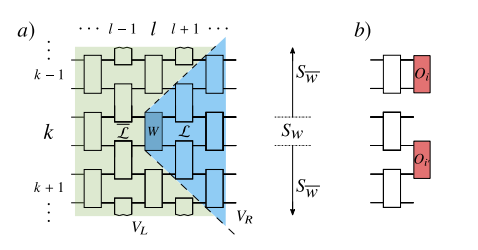
\includegraphics[scale=0.5]{LiteratureReview/Appendices/alterlayeransatz.png}
    \caption{
        Altering Layered Ansatz. 
        a) Each parameterized block $W_{kl}$ acts on $m$ qubits.
        $S_k$ is the $m$ qubit subsystem on which $W_{kL}$ acts, note that L is the last layer of the ansatz $U(\theta)$.
        The right (or forward) light-cone $\mathcal{L}$ contains all the gates with at least one input to $W$, $\overline{\mathcal{L}}$ is the opposite.
        $S_w$ is the subsystem of $m$ qubits which $W$ acts on, and $S_{\overline{w}}$ is the subsystem of $m$ qubits which $W$ have limited connection.
        b) The example of operator $O_i$ acts non-trivially in the subsystem $S_{k-1}$ only, while the operator $O_{i'}$ acts non-trivially on the second half ($m/2$) qubits of $S_k$ and on the first half ($m/2$) qubits of $S_{k+1}$.
        Figure from Cerezo et al. \cite{cerezoCostFunctionDependent2021}
    }
    \label{Altering Layered Ansatz}
\end{figure}

The authors introduced the \emph{altering layered ansatz} $U(\theta)$ with $L$ layers of $m$-qubit unitaries $W_{kl}(\theta_{kl})$ (see Figure \ref{Altering Layered Ansatz}).
If a local cost function is used for this altering layered ansatz, then there is a lower bound for the variants of the gradients that depend on the number of qubits and some circuit configurations. 
For a $L$-layered ansatz, let the variance $\mathrm{Var}[\partial_v C]$ of the partial derivative of the cost function $C$, the lower bound $G_n$ for the variance is:
\begin{equation}
    G_n(L,l) \leq \mathrm{Var}[\partial_k C]
\end{equation}
\begin{equation}
    G_n(L,l) = \frac{{2}^{m(l+1)-1}}{{({2}^{2m}-1)}^{2}{({2}^{m}+1)}^{L+l}}
    \times \mathop{\sum}\limits_{i\in {i}_{{\mathcal{L}}}}\mathop{\sum}\limits _{{(k,k^{\prime} )\in {k}_{{{\mathcal{L}}}_{\text{B}}}}\atop {k^{\prime} \geqslant k}}{c}_{i}^{2}\epsilon ({\rho }_{k,k^{\prime} })\epsilon ({\widehat{O}}_{i})\ ,
\end{equation}
Where the forward light-cone $\mathcal{L}$ is a set of gates with at least one input connected to the output of a block $W$; 
$S_k$ is the $m$-qubit subsystem;
$i_{\mathcal{L}}$ is a set of indices such that the operators $\hat{O_i}$ act on qubits in $\mathcal{L}$;
$k_{\mathcal{L}_B}$ is a set of indices such that the subsystem $S_k$ in the backward light-cone $\mathcal{L}_\text{B}$ of block $W$ (see Figure \ref{Forward-backward light cone} for example).
\begin{figure}
    \centering
    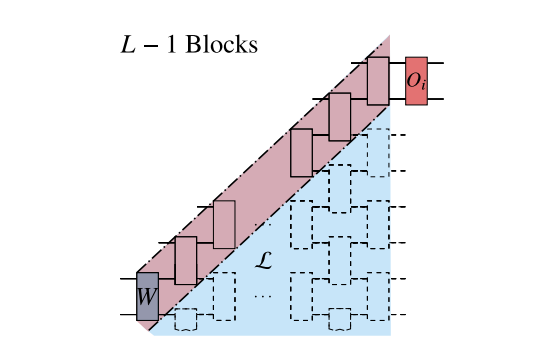
\includegraphics[scale=0.5]{LiteratureReview/Appendices/lightcone.png}
    \caption{
        An illustrative example of backward and forward light-cone.
        The operator $O_i$ in the topmost is in the scope of the forward light-cone $\mathcal{L}$ of block $W$.
        The thick-line dashes indicate the backward light-cone $\mathcal{L}_{\text{B}}$ of the operator $O_i$.
        Figure from Cerezo et al. \cite{cerezoCostFunctionDependent2021}
    }
    \label{Forward-backward light cone}
\end{figure}

If the total depth $L$ is in the range $O(\log(n))$ of the number of qubits (a shallow configuration), then the lower bound cannot vanish faster than $\Omega(1/\mathrm{poly}(n))$. 
Thus, no barren plateau occurs in this case.



\subsubsection{Layerwise learning}

There is another method that manipulates the circuit depth throughout the training period studied by Skolik et al. \cite{skolikLayerwiseLearningQuantum2021}. 
In more detail, the algorithm consists of two phases:

\textbf{\emph{The first phase}} constructs the ansatz by adding layers one by one, with all parameters initially set to zero. For a small number $s$ of starting layers, the set of parameters $\vec{\theta_1}$, and $W$ operators connecting qubits, then the initial layers $l_1(\vec{\theta_1})$ is presented:

\begin{equation}
    l_1(\vec{\theta_1})
    = \prod_{j=1}^s U_{1_j}(\vec{\theta_{1_j}}) W \;,
\end{equation}

Where each successive layer $l_i(\vec{\theta_i})$ of the form
\begin{equation}
    l_i(\vec{\theta_i})
    =U_i(\vec{\theta_i}) W \;,
\end{equation}
is added after repeated updates of the circuit parameters, at which point the parameters of all the previous layers become fixed. 
The process responsible for updating all circuit trainable parameters is called an \emph{iteration}. One \emph{epoch} is the number of iterations necessary for the algorithm to process each training sample.

This process can stop when a certain circuit depth is reached or until the objective function's value does not improve with additional layers.
Figure \ref{ll circuit} provides an illustrative example of the final circuit.
Eventually, we obtain the final circuit of $L$ layers:

\begin{equation}
    U(\vec{\theta})
    = \prod_{i=0}^L l_i (\vec{\theta_i}) \;.
\end{equation}
\begin{figure} 
    \centerline{
        \Qcircuit @C=1em @R=0em {
        & \multigate{4}{l_1(\vec{\theta_1})}    & \multigate{4}{l_2(\vec{\theta_2})}    & \qw &        & & \multigate{4}{l_i(\vec{\theta_i})}   & \qw\\
        & \ghost{l_1(\vec{\theta_1})}           & \ghost{l_2(\vec{\theta_2})}           & \qw &        & & \ghost{l_i(\vec{\theta_i})}          & \qw\\
        & \ghost{l_1(\vec{\theta_1})}           & \ghost{l_2(\vec{\theta_2})}           & \qw & \cdots & & \ghost{l_i(\vec{\theta_i})}          & \qw\\
        & \ghost{l_1(\vec{\theta_1})}           & \ghost{l_2(\vec{\theta_2})}           & \qw &        & & \ghost{l_i(\vec{\theta_i})}          & \qw\\
        & \ghost{l_1(\vec{\theta_1})}           & \ghost{l_2(\vec{\theta_2})}           & \qw &        & & \ghost{l_i(\vec{\theta_i})}          & \qw\\
        }
    }
    \caption{
        Constructing the ansatz from shallow layers.
    }\label{ll circuit}
\end{figure}


\textbf{\emph{The second phase}} takes the pre-trained circuit from phase one and trains larger adjacent partitions of layers at a time.
In more detail, we can set a parameter $r$ to specify the proportion of parameters to be trained in one step, e.g. one sixth, or one fifth the circuit layers.